\chapter{Support Vector Machines}

Support Vector Machines (SVMs) are a type of model used for both classification and regression. They used to be the most popular approach for supervised learning when there's little to no domain knowledge for the data, but they've been mostly replaced by neural networks and random forests.

\section{Hard Margin SVM}

Assume a classification task. Given a training set $TR = <x_i,d_i>, \, i=1 \dots N$, we want to find an hyperplane of equation $w^T x + b = 0$ to separate the examples; specifically, we want:

\begin{gather*}
    w^T x_i + b \geq 0 \text{ for } d_i = +1 \\
    w^T x_i + b < 0 \text{ for } d_i = -1
\end{gather*}

$g(x) = w^T x + b$ is called the \textbf{discriminant function}, and $h(x) = sign(g(x))$ is the hypothesis. Note that here the bias is referred to as $b$ instead of $w_0$. To find the hyperplane that separates all the points, instead of simply minimizing the empirical risk, the SVM minimizes the expected generalization error by finding the separator that is farthest away from all the examples in the dataset. It also establishes a margin ($\rho$) around it, whose width is exactly twice the distance between the hyperplane and the closest data point(s). The optimal hyperplane is the one that maximizes this margin $\rho$: $w_o^Txv + b_o = 0$, where $\rho = 2 / \|w_o\|$.

The two terms $w$ and $b$ can be rescaled so that the closest points to the separating hyperplane satisfy $\|g(x)\| = 1$, so we can write:

\begin{gather*}
    w^T x_i + b \geq 1 \text{ for } d_i = +1 \\
    w^T x_i + b < -1 \text{ for } d_i = -1 \, ,
\end{gather*}
or, in a compact form,
\begin{gather*}
    d_i(w^T x_i + b) \geq 1 \, .
\end{gather*}

Any $x_i$ that satisfies this equation is called a \textbf{support vector}, and is referred to as $x^{(s)}$. Let's denote the distance between the optimal hyperplane and a point $x$ as $r$, such that $x = x_p + r\frac{w_o}{\|w_o\|}$ (where $x_p$ is a point on the hyperplane). Evaluating $g(x)$ we obtain:

\begin{align*}
    g(x) = g(x_p + r\dfrac{w_o}{\|w_o\|}) = \\
    = w_o^Tx_p + b_o + w_o^T r \dfrac{w_o}{\|w_o\|} = \\
    = g(x_p) + w_o^T r \dfrac{w_o}{\|w_o\|} = \\
    = 0 + r \dfrac{\|w_o\|^2}{\|w_o\|} = r \|w_o\| \, ,
\end{align*}
thus, $r = \dfrac{g(x)}{\|w_o\|}$.

Consider the distance between the hyperplane and a positive support vector $x^{(s)}$, then $r$ is calculated as:

\begin{equation*}
    r = \dfrac{g(x^(s))}{\|w_o\|} = \dfrac{1}{\|w_o\|} = \dfrac{\rho}{2} \, ,
\end{equation*}
therefore, $\rho = \dfrac{2}{\|w_o\|}$.

\subsection{Primal Problem}

The optimum hyperplane will maximize $\rho$ and minimize $\|w\|$. One approach to find it is to perform a gradient descent to find the $w$ and $b$ that minimize/maximizes them, but there's another approach, that is solving a \textbf{quadratic optimization problem}.

\BoxDef{Quadratic optimization problem (primal form)}{
Given the training examples $TR = < x_i,d_i >$, find the optimal values of $w$ and $b$ which minimize
\begin{equation*}
    \Psi (w) = \dfrac{1}{2}w^T w
\end{equation*}
satisfying the constraints
\begin{equation*}
    d_i(w^T x_i + b) \geq 1 \, .
\end{equation*}
}
The objective function $\Psi (w)$ is quadratic and convex in $w$. The constraints are linear in $w$, and solving the problem scales with the size of the input space $m$.

To solve this problem, the \textbf{Lagrangian multipliers method} is used. The Lagrangian function corresponding to the quadratic optimization problem is constructed:
\begin{equation*}
    J(w,b,\alpha) = \dfrac{1}{2}w^T w - \sum_{i=1}^N \alpha_i(d_i(w^T x_i + b) - 1) \, ,
\end{equation*}
where $\alpha_i \geq 0$ are the \textbf{Lagrangian multipliers}. Each term in the sum corresponds to a constraint of the primal problem; $J$ must be minimized with respect to $w$ and $b$ and maximized with respect to $\alpha$. The solution will correspond to a saddle point of $J$.

If we minimize $J$ with respect to $w$, then:
\begin{gather*}
    \dfrac{\partial J}{\partial w} = \dfrac{2}{2} w - \sum_{i=1}^N \alpha_i(d_i(1*x_i + 0) + 0) = \\
    = w - \sum_{i=1}^N \alpha_i(d_i(x_i)) = 0
\end{gather*}
so
\begin{equation*}
    w = \sum_{i=1}^N \alpha_i(d_i(x_i)) \, .
\end{equation*}
Thus the optimal hyperplane is expressed as:
\begin{gather*}
    g(x) = w_o^T x + b_o = 0 \\
    \iff \\
    \sum_{i=1}^N \alpha_{o,i} d_i x_i^T x + b_o = 0 \, .
\end{gather*}
If instead we minimize it with respect to $b$:
\begin{gather*}
    \dfrac{\partial J}{\partial b} = 0 - \sum_{i=1}^N \alpha_i d_i = 0 \, .
\end{gather*}
These can be substituted in $J$ to study the dual form of the problem.

From the \textbf{Kuhn-Tucker Conditions}, it follows that
\begin{equation*}
    \alpha_i (d_i (w^T x_i + b) - 1) = 0 \, , \forall i = 1, \dots , N
\end{equation*}
in the saddle point of $J$. If $\alpha_i > 0$, then $(d_i (w^T x_i + b) = 1$, and $x_i$ is a support vector. If $x_i$ is not a support vector, then $\alpha_i = 0$. Hence we can restrict the computation to $N_s : w_o = \sum_{i=1}^{N_s} \alpha_{o,i} d_i x_i$. The hyperplane depends only on support vectors.

\subsection{Dual Problem}

To obtain the Lagrangian multipliers $\alpha_i$, we solve the problem in its dual form:

\BoxDef{Quadratic optimization problem (dual form)}{
Given the training examples $TR = < x_i,d_i >$, find the optimal values of $\alpha_i$ which maximize
\begin{equation*}
    Q(\alpha) = \sum_{i=1}^N \alpha_i - \dfrac{1}{2} \sum_{i=1}^N \sum_{j=1}^N \alpha_i \alpha_j d_i d_j x_i^T x_j
\end{equation*}
satisfying the constraints
\begin{gather*}
    \alpha_i \geq 0 \, , \forall i = 1, \dots , N \, ,\\
    \sum_{i=1}^N \alpha_i d_i = 0 \, .
\end{gather*}
}
The value of $\alpha_i$ can be found by solving the quadratic programming (QP) problem, or by more recent and efficient approaches (such as sequential minimal optimization (SMO)). Solving this problem scales with the number of training examples, less with the dimensionality. To find $w_o$ and $b_o$, we proceed as follows:
\begin{gather*}
    w_o = \sum_{i=1}^N \alpha_{o,i} d_i x_i \\
    b_o = 1 - w_o^T x^{(s)} = 1 - \sum_{i=1}^N \alpha_{o,i} d_i x_i^T x^{(s)} \, .
\end{gather*}
How do we use all of this? We don't actually need to explicitly know $w_o$. All we need are calculating the Lagrangian multipliers by solving the dual problem, and then calculating $b_o$. So, given the input pattern $x$, we compute $g(x) = \sum_{i=1}^N \alpha_{o,i} d_i x_i^T x + b_o$, and classify it as $h(x) = sign(g(x))$. Minimizing the norm of $w$ is equivalent to minimizing the VC-dim and VC-confidence of the model.

\BoxDef{Theorem - Vapnik}{
Let $D$ be the diameter of the smallest ball around the data points $x_1 , \dots , x_N$. For the class of separating hyperplanes described by the equation $w^T x + b = 0$, the upper bound to the VC-dim is
\begin{equation*}
    VC \leq min(\lceil \dfrac{D^2}{\rho^2} \rceil, m_0) + 1 \,,
\end{equation*}
where $m_0$ indicates the dimensionality of the input space.
}
Since $D^2 / \rho^2 = Radios^2 \|w\|^2$, VC can be less than $m_0 + 1$ computed for general hyperplanes by constraining the search to the ``regularized'' one with maximum margin.

This approach of finding optimal separating hyperplane maximizing the margin also provides:
\begin{itemize}
    \item An unique solution with zero errors for the binary classifier;
    \item An automatized approach to Structural Risk Minimization that minimizes the VC-confidence without having to deal with hyperparameters;
    \item The use of a solver in the class of constrained quadratic programming (instead of gradient descent) with a nice dual form;
    \item A solution focused on a selection of training data points: the support vectors.
\end{itemize}
But what about noisy or non linearly separable data?

\section{Soft Margin SVM}

In realistic datasets, the training set is not going to be perfect. It will contain noisy points and outliers that make the problem not linearly separable. The solution is to find a separator with a soft margin, that is, a margin that allows some errors within it. Because the margin can allow points to fall inside of it, the support vectors are no longer going to be the closest points to the margin.

We introduce what are called \textbf{slack variables}, which are non negative scalar variables:

\begin{gather*}
    \xi_i \geq 0 \, , \forall i = 1, \dots , N \\
    d_i(w^T x_i + b) \geq 1 - \xi_i \, , \forall i = 1, \dots , N
\end{gather*}
If $x^{(s)}$ is a support vector, it will satisfy the equation:
\begin{equation*}
    d_i(w^T x^{(s)} + b) = 1 - \xi_i 
\end{equation*}
Here, Vapnik's theorem does not hold anymore. The problem can be then rewritten to admit points in the margin.

\BoxDef{Quadratic optimization problem with Soft Margin (primal form)}{
Given the training examples $TR = < x_i,d_i >$, find the optimal values of $w$ and $b$ which minimize
\begin{equation*}
    \Psi(w, \xi) = \dfrac{1}{2}w^T w + C \sum_{i=1}^N \xi_i
\end{equation*}
satisfying the constraints
\begin{gather*}
    d_i (w^T x_i + b) \geq 1 - \xi_i \, , \forall i = 1, \dots N \\
    \xi_i \geq 0 \,, \forall i = 1, \dots N
\end{gather*}
}
The term $C$ is a user-defined regularization hyperparameter; so this version of SVM is no longer ``automatic'' like hard margin SVM was. $C$ is found as the trade-off between empirical risk minimization and capacity term (VC-confidence). If $C$ is too low, we allow many training errors, leading to underfitting. If $C$ is too high, we don't let any training error, leading to overfitting.

\BoxDef{Quadratic optimization problem with Soft Margin (dual form)}{
Given the training examples $TR = < x_i,d_i >$, find the optimal values of $\alpha_i$ which maximize
\begin{equation*}
    Q(\alpha) = \sum_{i=1}^N \alpha_i - \dfrac{1}{2}\sum_{i=1}^N \sum_{j=1}^N \alpha_i \alpha_j d_i d_j x_i^T x_j
\end{equation*}
satisfying the constraints
\begin{gather*}
    0 \leq \alpha_i \leq C \, , \forall i = 1, \dots , N \\
    \sum_{i=1}^N \alpha_i d_i = 0
\end{gather*}
}
The Kuhn-Tucker conditions can be redefined as:
\begin{gather*}
    \alpha_i (d_i (w^T x_i + b) + \xi_i - 1) = 0 \, , \forall i = 1, \dots , N \\
    \mu_i \xi_i = 0 \,, \forall i = 1, \dots , N \, ,
\end{gather*}
where $\mu_i$ are Lagrange multipliers introduced to enforce non-negativity of the slack variables in the primal function. If $0 < \alpha_i < C$, then $\xi_i = 0$. If $\alpha = C$, then $\xi_i \geq 0$. To solve the problem, we again solve the dual problem with respect to $\alpha_i$, and calculate $w_o$ and $b_o$ exactly as before.

\section{Mapping To a High-dimensional Space}

\href{https://en.wikipedia.org/wiki/Cover%27s_theorem#The_Theorem}{If the TR set represents a non-linearly separable problem, the data points can be mapped from the input space to a high-dimensional \textbf{feature space}, where they are linearly separable}. The approach we follow is analogous to the LBE for linear models. We define some function $\phi : \mathbb{R}^{m_0}\xrightarrow{} \mathbb{R}^{m_1}$. Finding this function, however, is not always easy, unless we have some prior knowledge allowing us to select the proper feature space. Also, using high dimensional feature spaces can lead to overfitting.

Given this function, we map all points to the new feature space: $x \mapsto \phi(x)$. The problem is formulated as before, with a new training set $TR = < \phi(x_i),d_i >$, and a new hyperplane $g(x) = w^T \phi(x) + b = 0$. The notation used here incorporates the bias in the weight vector, with $w_0 = b$ and $\phi_0(x) = 1$:
\begin{equation*}
    \phi(x) = (\phi_0(x) = 1, \phi_1(x), \dots , \phi_{m_1}(x))^T
\end{equation*}
The weight vector is now a linear combination of the feature vectors:
\begin{equation*}
    w = \sum_{i=1}^N \alpha_i d_i \phi(x_i)
\end{equation*}
and the hyperplane equation can be written as:
\begin{equation*}
    g(x) = \sum_{i=1}^N \alpha_i d_i \phi^T (x_i) \phi(x) = 0
\end{equation*}
Evaluating $\phi(x)$ may be intractable. Fortunately, under certain conditions we do not need to evaluate it directly, or even know the feature space itself. This is possible with a so-called \textbf{kernel trick}, i.e. by using a function $k$ to directly compute the dot products $\phi^T (x_i) \phi(x)$ in the feature space:
\begin{equation*}
    k : \mathbb{R}^{m_0} \times \mathbb{R}^{m_0} \xrightarrow{} \mathbb{R}
\end{equation*}
This function is known as the \textbf{inner product kernel function}. It's also a symmetric function, so $k(x_i, x) = k(x, x_i)$. Consider the function $\phi(x) = \phi((x_1, x_2)^T) = (x_1^2, \sqrt{2}x_1x_2, x_2^2)^T$. Given $x = (x_1, x_2)^T$ and $y=(y_1,y_2)^T$ in $\mathbb{R}^2$, we compute $\phi^T(x)\phi(y)$ in this 
\begin{gather*}
    \phi^T(x)\phi(y) = (x_1^2, \sqrt{2}x_1x_2, x_2^2) (y_1^2, \sqrt{2}y_1x_2, y_2^2)^T = \\
    x_1^2y_1^2 + 2x_1y_1x_2y_2 + x_2^2y_2^2 = (x_1y_1 + x_2y_2)^2 = \\
    ((x_1,x_2)(y_1,y_2)^T)^2 = (x^Ty)^2 = k(x,y)
\end{gather*}
We can arrange the dot products in the feature space between the img of the input training patterns in a $N$ by $N$ matrix, called \textbf{kernel matrix}:
\begin{equation*}
    K = \begin{pmatrix}
        k(x_1,x_1) & \dots & k(x_1, x_N) \\
        k(x_2,x_1) & \dots & k(x_2, x_N) \\
        \vdots & & \vdots \\
        k(x_N,x_1) & \dots & k(x_N, x_N) \\
        \end{pmatrix} \,, \,
        K = \{k(x_i, x_j)\}_{(i,j)=1)}^N
\end{equation*}
The kernel matrix is symmetrical, as the inner product kernel is symmetrical. Not every kernel function computes the inner product in a feature space; this property holds only for kernels gaining positive semi-definite kernel matrices. This is related to the matrix having non negative Eigenvalues.

Given $k_1$ and $k_2$ both kernels over $\mathbb{R}^{m_0} \times \mathbb{R}^{m_0}$. The following are also kernel functions:
\begin{itemize}
    \item $k_1(x,y) + k_2(x,y)$;
    \item $\alpha k_1(x,y) \, \forall \alpha \in \mathbb{R}_+$;
    \item $k_1(x,y)k_2(x,y)$.
\end{itemize}

The problem is reformulated in both forms as follows.

\BoxDef{Quadratic optimization problem in feature space (primal form)}{
Given the training examples $TR = < \phi(x_i),d_i >$, find the optimal values of $w$ which minimizes
\begin{equation*}
    \Psi(w, \xi) = \dfrac{1}{2}w^T w + C \sum_{i=1}^N \xi_i
\end{equation*}
satisfying the constraints
\begin{gather*}
    d_i (w^T \phi(x_i)) \geq 1 - \xi_i \, , \forall i = 1, \dots N \\
    \xi_i \geq 0 \,, \forall i = 1, \dots N
\end{gather*}
}

\BoxDef{Quadratic optimization problem in feature space (dual form)}{
Given the training examples $TR = < \phi(x_i),d_i >$, find the optimal values of $\alpha_i$ which maximize
\begin{equation*}
    Q(\alpha) = \sum_{i=1}^N \alpha_i - \dfrac{1}{2}\sum_{i,j=1}^N \alpha_i \alpha_j d_i d_j k(x_i,x_j)
\end{equation*}
satisfying the constraints
\begin{gather*}
    \sum_{i=1}^N \alpha_i d_i = 0 \\
    0 \leq \alpha_i \leq C \,, \forall i = 1, \dots N
\end{gather*}
}
Remember that C is a user specified non-negative  regularization hyperparameter.

To classify an unseen input pattern $x$ using the machine we trained, we compute $\sum_i \alpha_i d_i k(x, x_i)$, and then classify $x$ as $h(x) = sign(\sum_{i=1}^n \alpha_i d_i k(x, x_i))$. Note: we have to memorize the $x_i$ in the training set for the test phase.

Some examples of commonly used kernels include:
\begin{itemize}
    \item \textbf{Polynomial Learning Machine}: $k(x,x_i) = (x^T x_i + 1)^p$ (where $p$ is a user-specified parameter);
    \item \textbf{Radial Basis Function Net}: $k(x, x_i) = e^{-\frac{\|x - x_i\|^2}{2 \sigma^2}}$ (where $\sigma$ is a user-specified parameter);
    \item \textbf{Two-layer Perceptron}: $k(x,x_i) = tanh(\beta_0 x^T x_i + \beta_1)$ (where $\beta_0 > 0$ and $\beta_1 < 0$ are user-specified parameters).
\end{itemize}

For the first two kernels, we always get an inner product kernel, but for a two-layer perceptron the values of $\beta_0$ and $\beta_1$ must be chosen carefully to ensure we have the appropriate kernel. Also, using a kernel function of type RBF always leads to a feature space with an infinite number of dimensions.

\section{SVMs For Nonlinear Regression}

Earlier, we defined a task by specifying that the TR set contains a number of inputs and corresponding labels. Each label $d_i = f(x) + v$, i.e., is equal to the output value of the (unknown) target function plus a certain noise disturbance. This noise term $v$ is statistically independent from $x$.

To estimate the regression output $y$ using a linear expansion of non-linear functions:
\begin{equation*}
    y = h(x) = w^T\phi(x) \,,
\end{equation*}
where $w = (w(0)=1, w(1), \dots , w(m_1))^T$ and $\phi(x) = (\phi_0(x)=1, \phi_1(x), \dots , \phi_{m_1}(x))^T$.

For SVMs, the loss function used is called \textbf{$\epsilon$-insensitive loss function}, and is defined as:
\begin{equation*}
    L_{\epsilon}(d,y) = \begin{cases}
                        |d-y| - \epsilon & \text{if } |d-y| \geq \epsilon \\
                        0 & \text{otherwise}
                        \end{cases}
\end{equation*}

\begin{figure}[h]
    \centering
    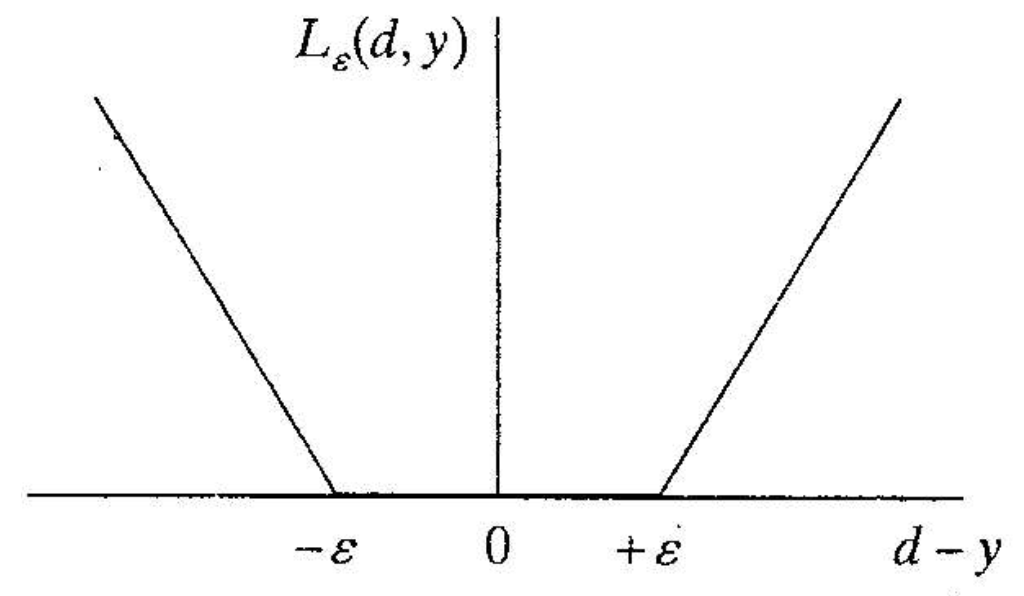
\includegraphics[width=0.5\linewidth]{img/epsiloninsensitive.png}
\end{figure}
By plotting the function and the resulting margin, the $\epsilon$-tube is constructed. (?)

To formulate the optimization problem for regression, we must first introduce two sets of slack variables, $\xi_i'$ and $\xi_i$, such that:
\begin{equation*}
    -\xi_i' - \epsilon \leq d_i - w^T\phi(x_i) \leq \epsilon + \xi_i \,, \forall i = 1, \dots , N
\end{equation*}
We can now formulate the primal and dual problems for regression.

\BoxDef{Quadratic optimization problem for regression (primal form)}{
Given the training set TR = $<x_i, d_i>$, find the optimal values of $w$ which minimize
\begin{equation*}
    \Psi (w,\xi,\xi') = \dfrac{1}{2}w^T w + C \sum_{i=1}^N (\xi_i + \xi_i')
\end{equation*}
satisfying the following constraints
\begin{gather*}
    -\epsilon - \xi_i' \leq d_i - w^T\phi(x_i)  \leq \epsilon + \xi_i \\
    \xi_i \geq 0 \\
    \xi_i' \leq 0
\end{gather*}
}

\BoxDef{Quadratic optimization problem fr regression (dual form)}{
Given the training set TR = $<x_i,d_i>$, find the optimal values of $\alpha_i$ and $\alpha'$ which maximize
\begin{equation*}
    Q(\alpha, \alpha') = \sum_{i=1}^N d_i(\alpha_i - \alpha_i') - \epsilon \sum_{i=1}^N \alpha_i + \alpha' - \dfrac{1}{2}\sum_{i,j=1}^N (\alpha_i - \alpha_i')(\alpha_j - \alpha_j')k(x, x_i)
\end{equation*}
satisfying the following constraints
\begin{gather*}
    \sum_{i=1}^N \alpha_i - \alpha_i' = 0 \\
    0 \leq \alpha_i \leq C \\
    0 \leq \alpha_i' \leq C
\end{gather*}
}
Again, solving the dual problem gives us the best values of $\alpha_i$ and $\alpha_i'$, and then we compute the weight vector:
\begin{equation*}
    w = \sum_{i=1}^N (\alpha_i - \alpha_i')\phi(x_i) \iff w = \sum_{i=1}^N \gamma_i \phi(x_i)
\end{equation*}
In this case, the support vectors correspond to non-zero values of $\gamma_i$.

So, the estimate function can be expanded accordingly:
\begin{align*}
    h(x) = y = w^T \phi(x) = \\
    = \sum_{i=1}^N \gamma_i \phi(x_i) \phi(x) = \\
    = \sum_{i=1}^N \gamma_i k(x_i,x) \,.
\end{align*}

\section{Pros and Cons of SVM}

\textbf{Pros:}
\begin{itemize}
    \item The regularization is embedded within the optimization problem, so it does not need any external hyperparameter for it;
    \item It automatically approximates SRM by finding the hypothesis with the best possible VC-dim;
    \item It's a convex problem, so the global minimum can always be found;
    \item Features are implicitly transformed through kernels;
    \item Linear model with bound of the  complexity that depends on the margin (which is optimized);
    \item Rich set of non-linear decision functions in the input space via kernels.
\end{itemize}

\textbf{Cons:}
\begin{itemize}
    \item Kernel and kernel parameters must be chosen explicitly;
    \item It uses a batch algorithm to update the weights, so no chance to parallelize;
    \item Very large problems were computationally intractable (although nowadays many efficient solutions have been proposed, including gradient descent ones);
    \item For soft margin SVM, since we have to select the $C$ parameter and the kernel function, we have no guarantee that the final model will have high accuracy.
\end{itemize}

Note that for the last point about soft margin, the VC-dim of the model is controlled by the width of the margin. If we choose the smallest possible margin (with just one support vector), we can classify an arbitrarily large number of training points correctly, thus the VC-dim will be infinite. If instead we have a very large width, we end up in a situation where all points in the TR set are used as support vectors, therefore leading to a low VC-dim. This is analogous to using a k-NN classifier with $k=1$ and $k=l$, respectively. Also, the hyperparameter $C$ used for regularization must be chosen appropriately for the kernel hyperparameters, so cross-validation is needed.

\section{Kernel Methods}

In general, \textbf{kernelization} of an approach is done by substituting a dot product or similarity measure in a model with a kernel function that maps to an high-dimensional space.

$K(s,t)$ can be related to a similarity measure, comparing $s$ and $t$; e.g.:
\begin{equation*}
    d_k(s,t) = \sqrt{k(s,s) - 2k(s,t) + k(t,t)}
\end{equation*}
If the objects are similar (so the distance is small) the kernel will have high value. The focus is on the idea that in some situations, it's easier to focus on simplifying pairwise comparison by doing it in a different space rather than the representation of the single object.

The best choice of kernel for a given problem is still a research issue.